% Performance testing +- same performance
% https://ieeexplore.ieee.org/abstract/document/8928192

% Performance testing +monolith
% https://ieeexplore.ieee.org/abstract/document/9109514

So far we have looked at three different types of architectural patterns. In this chapater we will look at the implementation of a simple application using all 3 architectural patterns discussed (Monolith, Mudulith, Microservice). We will look at the implications in terms of internal structure, database design, scalability and of course performance.

\section{Application}
This is an application example of a real world system consisting of HTTP API, database queries and business logic. It has been designed to be easy to understand and to solve a problem known to everyone: orders. Each application exposes the following HTTP API:
\begin{itemize}
    \item \textbf{Get /item} - Retrieve all existing items.
    \item \textbf{Get /item/\{itemId\}} - Retrieve an existing item specified by id.
    \item \textbf{Post /cart/items/\{itemId\}} - Add item to shopping cart.
          % \item \textbf{Delete /cart/items/\{itemId\}} - Remove item from shopping cart.
    \item \textbf{Post /order/create} - Create an order from items in shopping cart.
    \item \textbf{Get /order/\{orderId\}} - Retrieve order specified by id.
          % \item \textbf{Post /order/\{orderId\}/cancel} - Cancel order specified by id.
    \item \textbf{Get /invoice/\{invoiceId\}} - Retrieve invoice specified by id.
    \item \textbf{Get /payment/\{paymentId\}} - Retrieve payment specified by id.
    \item \textbf{Post /payment/invoice/\{invoiceId\}} - Pay for invoice specified by id.
\end{itemize}

The Client of the application can view items, add them to his shopping cart, place an order, retrieve an invoice and pay for it. Like most of the applications today, there are mainly operations querying data or saving data into database. The activity flow is described on Figure~\ref{img:app_activity_flow}. First, a session is created for the client, then the client loads items and adds everything he wants to his shopping cart. Later the client places an order, an invoice is generated in the background and the client can cancel the order or pay for it. To add more CPU intensive tasks, invoice generates PDF and also calculates 41st Fibonacci number.

Candidates for the implementation programming language were Rust and Golang due to its minimal runtime (minimal impact on benchmarking). Winner is Golang because it's easier to use, good personal experience of the authors and better support for the Open Tracing project, which is used for monitoring from within the application during benchmarking. All applications are based on \textit{gorilla/mux} \cite{MUX} for http server + request routing library and \textit{Bun} \cite{BUN} as a lightweight ORM.

PostgreSQL was chosen as the data store because SQL databases are more widely known than NoSQL, so it should be easier for anyone to understand the design. It was chosen because of its current popularity and the authors' preference for it over MySQL.
\begin{figure}
    \centering
    \includesvg{images/app_activity.svg}
    \caption{Diagram describes client flow of application. \label{img:app_activity_flow}}
\end{figure}

The application needs to be able to run in multiple instances so that it can be properly benchmarked and scaled later. In order to run the application in multiple instances, a container orchestrator will need to be used. Instead of adding unnecessary complexity when using Kubernetes, I decided to use \textit{docker compose} to manage containers, as I do not plan to run the application on multiple nodes. All requests are sent to Nginx, which acts as both a reverse proxy and a load balancer.


\section{Monolith example}
This example is implemented as a monolithic system. Basically it is a three tier application: presentation (HTTP API), application and data (database). Figure~\ref{img:monolith_db_schema} describes the internal structure of the application packages. \textit{Routes} package contains path mapping for endpoint handlers defined in \textit{endpoints}. Handlers contain simple logic definition, more complex logic is in \textit{services} and data manipulation around the database is in \textit{database}.

% \begin{figure}
%     \centering
%     \includesvg[width=0.7\textwidth]{images/monolith_package.svg}
%     \caption{Internal package structure of Monolithic example. \label{img:monolith_package}}
% \end{figure}


\subsection{Database}
Due to the nature of Monolith as a unified system, all data resides within a single database, making full use of constraints and referential integrity, thus ensuring data consistency. Complete database schema is shown on diagram~\ref{img:monolith_db_schema} consisting of 7 tables, five of which are entity tables and two are entity relationship mapping. The application will have a database pool consisting of a maximum of 8 connections.

\begin{figure}
    \centering
    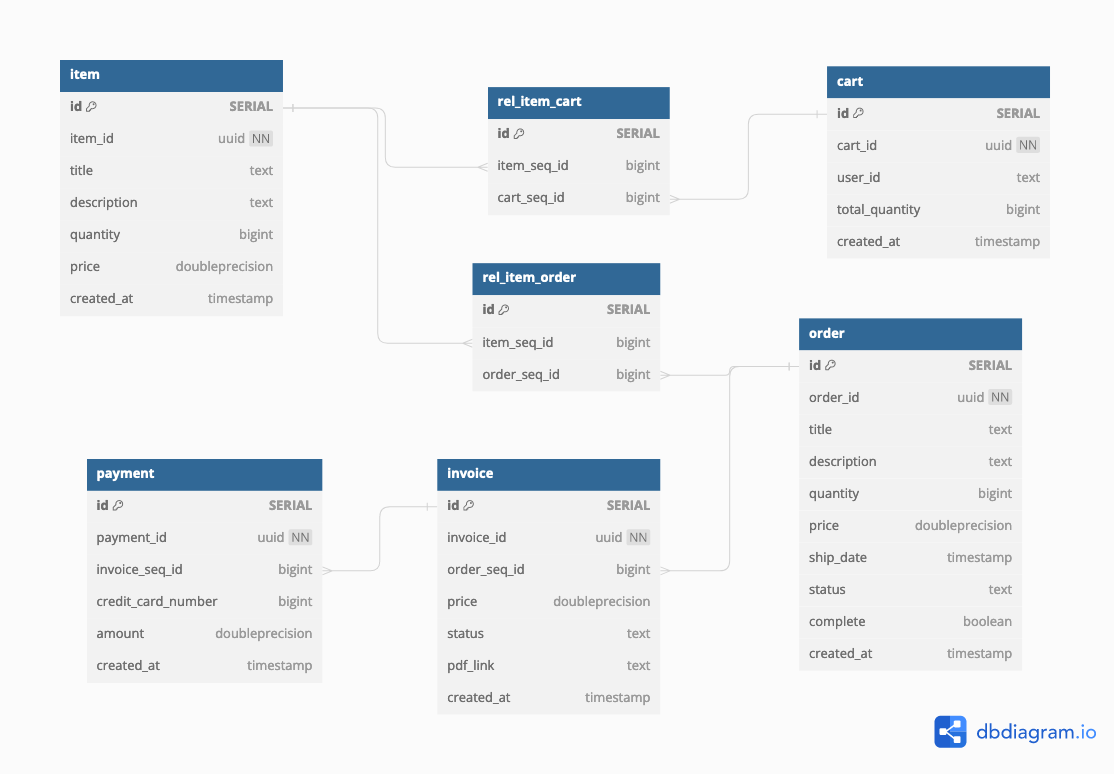
\includegraphics[width=\textwidth]{images/monolith_db_schema.png}
    \caption{Database schema displaying tables and relations of Monolithic example. \label{img:monolith_db_schema}}
\end{figure}



\section{Modulith example}
This is an example of using the modular monolith approach. The original monolithic application has been split into several smaller monoliths called \textit{modules}. The size of each module depends on the specificity of the project. In this case, it is almost equivalent to one module per database entity, except for the shopping cart and items, which have been merged into a single module to demonstrate the possibility of having modules with a larger volume. Package schema and dependencies are shown in diagram~\ref{img:modulith_package}.

Each module has the same internal structure as the original Monolith plus exposes its API with an interface (Diagram~\ref{img:modulith_module_package}). Modules encapsulate their own data storage, and there should be no cross-module table constraints in the database, although this is possible, it doesn't make sense from a logical separation perspective. It should be possible for each module to use a different database and even a different database technology. In the case of the largest module, which contains the shopping cart and items, foreign key constraints are preserved because it resides within a single module.

Modules can use API of other modules, although this should be limited as much as possible to keep coupling low. The dependency on other modules is defined through the use of interfaces, and the actual implementation can either be automatically injected using the IoC approach, or as in this case, just define a top level module that takes care of initialising individual modules and spinning up a single HTTP server.

Scaling Modulith once we have identified the bottleneck packages is very easy. Since each module is essentially a small monolith, it can be moved into service and run independently. It just needs to expose its API over the network, such as gRPC or just a simple HTTP API. This network exposure can be generated automatically if all objects in the interface are serialisable. Later client instances will be passed to all dependent modules and from the point of view of other modules nothing changes, only now the underlying communication will not be inter-process communication but network communication. The implementation could even be fully automated in a declarative way. The package can be moved to a separate service and scaled, simply by changing the configuration.

In this particular example, the implementation to expose the capabilities defined in the invoice interface was created manually by defining the following additional HTTP endpoints and thus implementing a client to satisfy the existing interface.

\begin{itemize}
    \item \textbf{Post /invoice} - Generate invoice for order specified in body.
    \item \textbf{Patch /invoice/\{invoiceId\}} - Update invoice specified by id.
\end{itemize}

The Modulith application has been extended to run in 3 modes, depending on the value of environment variables. In the first mode it runs as a single process. In the second mode it runs as a single process without invoice implementation and uses the invoice client. In the third mode it runs only the invoice implementation and this can be scaled to many instances to improve performance. Load balancing of requests to the invoice service instances is done using Nginx.

% \begin{figure}
%     \centering
%     \includesvg[width=0.7\textwidth]{images/modulith_module_package.svg}
%     \caption{Internal package structure of single module (Modulith example).\label{img:modulith_module_package}}
% \end{figure}

% \begin{figure}
%     \centering
%     \includesvg[width=0.7\textwidth]{images/modulith_package.svg}
%     \caption{Module dependency graph of Modulith example. \label{img:modulith_package}}
% \end{figure}

\subsection{Database}
Each module encapsulates its own tables, completely independent of the rest. The tables are the same as for the monolithic example on diagram~\ref{img:monolith_db_schema}, but the relations between modules have been removed. The schema consists of four partitions with relations preserved within the partition: the first partition consists of the invoice table, the second of the payment table, the third of the order table with rel\_item\_order and the last of the item, cart and rel\_item\_cart tables. Each module will have its own database pool with a maximum of 2 connections (8 in total).

% \begin{figure}
%     \centering
%     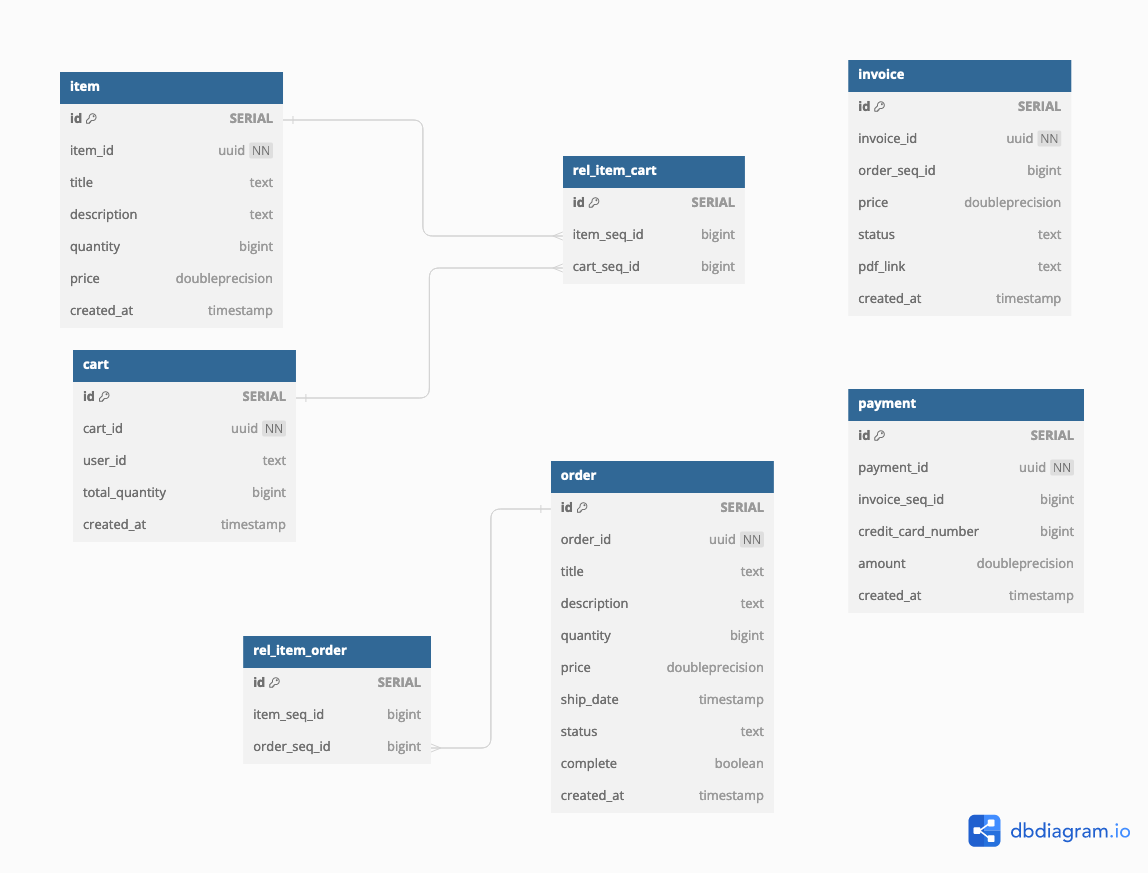
\includegraphics[width=\textwidth]{images/modulith_db_schema.png}
%     \caption{Database schema displaying tables and relations. \label{img:modulith_db_schema}}
% \end{figure}

\section{Microservices example}
In this example, the Modulith implementation has been further split into 5 microservices: Item, Shopping Cart, Invoice, Order and Payment. Modulith originally contained 4 packages, 1 of which combined the logic around Shopping Cart and Items, so it was split into two to make the scope more consistent across the microservices. The dependency graph between services is shown in Figure~\ref{img:microservices_dependency}.

Splitting Modulith into services requires exposing additional functionality over the network, as Modulith modules communicate with other modules via inter-process communication. As a result, additional endpoints (compared to the monolith) and clients had to be created to satisfy the defined interfaces.

% TODO přidat která další API musela vzniknout
\begin{itemize}
    \item \textbf{Post /invoice} - Generate invoice for order specified in body.
    \item \textbf{Patch /invoice/\{invoiceId\}} - Update invoice specified by id.
    \item \textbf{Delete /cart/\{cartId\}} - Remote cart specified by id.
    \item \textbf{Get /cart/\{cartId\}/item/id} - Retrieve item ids within cart.
    \item \textbf{Get /cart/user/\{userId\}} - Retrieve cart for user specified by user id.
\end{itemize}

Each microservice runs an HTTP server and exposes HTTP API for its internal API to be used by other modules and also public HTTP API to be used by clients. With microservices it is common to use some kind of service discovery and let services communicate directly with each other. In this example, to keep things simple, nginx was used as a load balancer, acting as an intermediary and directing requests to the right services by path matching.

The whole application is compiled into a single binary, but in production it would most likely be compiled into binaries per service. Which service is started is controlled by an environment variable.

% \begin{figure}
%     \centering
%     \includesvg[width=0.7\textwidth]{images/microservices_dependency.svg}
%     \caption{Dependency between microservices. \label{img:microservices_dependency}}
% \end{figure}

\subsection{Database}
Each microservice encapsulates its own data. The database tables are the same as for the monolithic example on diagram~\ref{img:monolith_db_schema}, but the constraints outside the microservice scope have been removed. Database partitions are the same as for Modulith, only item table has been separated into its own service after splitting one package into two separate: cart and item. Each microservice will have its own database pool with a maximum of 2 connections (10 in total).

\begin{figure}
    \centering
    \begin{subfigure}{.5\textwidth}
        \centering
        \includesvg[width=0.9\textwidth]{images/monolith_package.svg}
        \caption{Internal package structure of Monolith example. \label{img:monolith_package}}
    \end{subfigure}%
    \begin{subfigure}{.5\textwidth}
        \centering
        \includesvg[width=1\textwidth]{images/modulith_module_package.svg}
        \caption{Internal package structure of single module (Modulith example).\label{img:modulith_module_package}}
    \end{subfigure}
    % \vspace{0.5cm}
    \begin{subfigure}{\textwidth}
        \centering
        \includesvg[width=0.7\textwidth]{images/modulith_package.svg}
        \caption{Module dependency graph of Modulith example. \label{img:modulith_package}}
    \end{subfigure}%
    \hfill
    \begin{subfigure}{\textwidth}
        \centering
        \includesvg[width=0.7\textwidth]{images/microservices_dependency.svg}
        \caption{Dependency graph between services of Microservices example. \label{img:microservices_dependency}}
    \end{subfigure}
    \caption{Architecture diagrams for application examples build with architectures: Monolith, Modulith and Microservices.}
\end{figure}


\section{Benchmark methodology}
There are two types of scenarios, which will be measured to get inside into bottlenecks of applications from both CPU intensive and IO intensive perspective. Benchmarking will be done using K6 load testing tool, which will act as HTTP client sending requests defined by scenario.

Benchmarking will be done for following test scenarios with various configurations:
\begin{itemize}
    \item Performance scenario - focusing on even load of whole application testing IO and CPU intensive operations.
    \item Latency scenario - focusing primarily on IO operations and handling a lot of fast requests.
\end{itemize}

All benchmarks results will originate from running 10 parallel tests, totally 100 iterations with following configuration.
\begin{itemize}
    \item Golang 1.21.3 - programming language used for applications
    \item PostgreSQL 14 - database
    \item Docker 24.0.5 - execution environment
    \item OpenTelemetry - monitoring from within application
    \item k6 - load testing tool
    \item Hardware - Macbook Air 13" with M2, 16 GB Ram, 6 CPU cores assigned to Docker
          % TODO this configuration might change for MicroServices -> we will see
    \item Every service instance has following assigned resources unless specified otherwise: 0.5~CPU and 50~MB of Ram
\end{itemize}


\section{Benchmark results}
\label{section:benchmark_results}

\subsection{Performance scenario}
The first scenario consists of going through the whole application flow as defined on Figure~\ref{img:benchmark_flow}, which should represent evenly distributed load on the whole system. Client load list of houndred items and adds one random into his shopping cart. This repeats 10 times, after that client creates order, retrieves invoice information and pays for it. The application cosists of database queries and two harder jobs, which represents possible real world task. The first is CPU intensive task will be done during creation of order, where application generates PDF and also calculates 41st Fibonacci number to add more cpu load. The second big task, which represents waiting for 3rd party service is done during handling payment, which is implemented as 500~ms sleep.

\begin{figure}
    \centering
    \includesvg[width=0.7\textwidth]{images/benchmark_flow.svg}
    \caption{Benchmark flow diagram. \label{img:benchmark_flow}}
\end{figure}

In Table \ref{table:benchmark_baseline} are results of benchmark which will act as baseline. Both Monolith and Modulith were running in single instance with 0.5~CPU assigned and Microservices assigned 0.5~CPU per service. Even though both Monolith and Modulith are running as single process, there is already little overhead visible due to more complex internal structure and more database connection pools (separate database pool is created for every module).

\begin{table}
    \begin{tabular}{ |p{3cm}||p{3cm}|p{1.5cm}|p{1.5cm}|p{1.5cm}|p{1.5cm}| }
        \hline
        \multicolumn{5}{|c|}{Benchmark performance scenario}                           \\
        \hline
        Architecture  & Resources         & rps        & avg     & p(90)   & p(95)   \\
        \hline
        Monolith      & 0.5\,CPU, 50\,MB  & 6.8\,req/s & 1.43\,s & 1.2\,s  & 14.4\,s \\
        Modulith      & 0.5\,CPU, 50\,MB  & 7.8\,req/s & 1.25\,s & 1.59\,s & 9.18\,s \\
        Microservices & 2.5\,CPU, 250\,MB & 6.9\,req/s & 1.43\,s & 1.1\,s  & 17.9\,s \\
        \hline
    \end{tabular}
    \caption{Table containing benchmark results comparing Monolith, Modulith and Microservices. Microservices and much more CPU reserved, since it consist of 5 services (every singe one has 0.5~CPU assigned).\label{table:benchmark_baseline}}
\end{table}

The biggest bottleneck of first scenario is CPU bound task. To scale Monolith we would have to run more instances, which for big systems is very resource demanding, and target of this theses is to focus on more modern architecture styles, so it will not be discussed further. On the other hand for modulith systems it is much easier due to its modular structure. The cpu bound task is contained inside invoice package, which can be moved into separate lightweight service and scaled as much as wanted.

In second measurement invoice package was moved into separated service implementing HTTP server. HTTP client is than passed in main server to whoever module required the invoice interface. The same benchmark was run for one, two, four and eight instances of invoice service and results can be seen in Table~\ref{table:benchmark_modulith_instances} along with scaled Microservices example. There is no difference between Modulith and Modulith with single invoice service instance, but having the invoice service scaled to two instances, it has more then doubled the speed. Adding more instances scales linearly until the main bottleneck becomes IO bound task during payment. Microservices scale as well as Modulith, but having more overhead (more network inter-service communication) they are slightly slower.

\begin{table}
    \begin{tabular}{ |p{4cm}||p{1.6cm}|p{1.5cm}|p{1.5cm}|p{1.5cm}|p{1.5cm}| }
        \hline
        \multicolumn{5}{|c|}{Benchmark performance scenario}                                  \\
        \hline
        Architecture                & Resources & rps         & avg     & p(90)   & p(95)   \\
        \hline
        Modulith unified            & 0.5\,CPU  & 7.8\,req/s  & 1.25\,s & 1.59\,s & 9.1\,s  \\
        \rowcolor{Gray}
        Modulith (1x invoice)       & 1.0\,CPU  & 7.3\,req/s  & 1.35\,s & 1.0\,s  & 18.6\,s \\
        \rowcolor{Gray}
        Microservices (1x invoice)  & 2.5\,CPU  & 6.9\,req/s  & 1.43\,s & 1.1\,s  & 17.9\,s \\
        Modulith (2x invoice)       & 1.5\,CPU  & 18.8\,req/s & 510\,ms & 605\,ms & 3.1\,s  \\
        Microservices (2x invoice)  & 3.0\,CPU  & 21.4\,req/s & 441\,s  & 612\,ms & 3.9\,s  \\
        \rowcolor{Gray}
        Modulith (4x invoice)       & 2.5\,CPU  & 44.2\,req/s & 204\,ms & 521\,ms & 1.2\,s  \\
        \rowcolor{Gray}
        Microservices  (4x invoice) & 4.0\,CPU  & 58.3\,req/s & 165\,ms & 513\,ms & 1.0\,s  \\
        Modulith (8x invoice)       & 4.5\,CPU  & 71.6\,req/s & 133\,ms & 512\,ms & 0.8\,s  \\
        Microservices (8x invoice)  & 6.0\,CPU  & 66.4\,req/s & 142\,ms & 519\,ms & 0.9\,s  \\
        \hline
    \end{tabular}
    \caption{Table containing benchmark for Modulith and Microservices with module invoice moved into separate service running in multiple number of instances (indicated by number in parentheses).\label{table:benchmark_modulith_instances}}
\end{table}


\subsection{Latency scenario}
The second scenario consist just of the iterations part of previous scenario as defined on Figure~\ref{img:benchmark_flow}, but instead of repeating 10 times as in first scenario, it will repeat 100 times. Benchmark will send totally 2 000 requests (100 iterations of scenarios, 100 iterations in scenario, 2 requests per iteration), where handling of requests will consist of multiple database queries, so application will be most of the time waiting for network or database.

Benchmark will be running 100 iterations consisting of 3 http requests to retrieve list of items, add random item to shopping cart and later remove it from shopping cart. For Monolith and Modulith it is just matter of inter-process communication and database queries. In case of Microservices, there is overhead in network inter-service communication. To handle either add or remove item, there are two network requests involved: first to retrieve item data to validate if the id of item is valid and second request to load data for all item ids contained inside shopping cart.

Results of running benchmark scenario are in Table \ref{table:benchmark_scenario2}. After running initial tests, there was unexpected behavior of Monolith, which has been much slower compared to Modulith (367~req/s vs. 571~req/s). During inspecting the runtime behavior via gathered OpenTelemetry metrics, it was found out, that application used up all the available memory and was not able to process more parallel requests. Assigning it 100~MB of memory fix the issue, although it surprisingly still did not supersede the Modulith in terms of performance. Microservices had the worst performance even though they had assigned much more resources, but the benchmark is actively pressing only two microservices: cart and item, and there is the overhead of network communication between them, which has to go through the whole network stack compared to inter-process communication in other two examples. The network communication added in average 24~ms to every inter-service communication, which caused inevitable reduction in performance (four times compared to Modulith) - this metric has been measured during running benchmark using OpenTelemtry tracing.

This huge performance difference in Microservices was much more than what was initially expected around 10\,\%. After looking into tracing and resource usage statistics, the main bottleneck was evidently database, where execution time of queries ranged from hundreds microseconds up to more than 5 seconds. This has been a big surprise, since Modulith application is making exactly the same database queries, but the issue wasn't there. There came some database optimization in play where depending on order of queries database was able to optimize it and in case of Modulith application the order was just better.

\label{p:latency_issue}

\begin{table}
    \begin{tabular}{ |p{3cm}||p{3cm}|p{1.5cm}|p{1.5cm}|p{1.5cm}|p{1.5cm}| }
        \hline
        \multicolumn{5}{|c|}{Benchmark latency scenario}                                       \\
        \hline
        Architecture  & Resources         & rps        & avg    & p(90)    & p(95)   \\
        \hline
        \rowcolor{Gray}
        Monolith      & 0.5\,CPU, 50\,MB  & 367\,req/s & 6\,ms  & 51\,ms   & 67\,ms  \\
        Monolith      & 0.5\,CPU, 100\,MB & 546\,req/s & 6\,ms  & 60\,ms   & 75\,ms  \\
        \rowcolor{Gray}
        Modulith      & 0.5\,CPU, 50\,MB  & 571\,req/s & 6\,ms  & 68\,ms   & 75\,ms  \\
        Microservices & 2.5\,CPU, 250\,MB & 130\,req/s & 82\,ms & 107ms\,s & 173\,ms \\
        \hline
    \end{tabular}
    \caption{Table containing benchmark results comparing Monolith, Modulith and Microservices for second scenario.\label{table:benchmark_scenario2}}
\end{table}

All benchmarks were run on a single machine, where it does not properly demonstrate performance drawback of distributed system as Microservices are. Even though there is network communication, the latencies are pretty low compared to actually running on multiple nodes, which would add even more latency. To demonstrate this on single machine, Linux Traffic Control has been used, which is very useful Linux utility that gives ability to configure the kernel packet scheduler to modify any network property \cite{MAN_TRAFFIC_CONTROLL}. After spawning the containers the \textit{tc} command was used to set manually latency to all packets, which simulates real-world environment.

Table~\ref{table:benchmark_scenario2} contains benchmark results from running latency scenario with added extra latency to every running service. For modulith the extra latency is just on request coming from the client in both directions (inbound and outbound traffic). In case of microservices the extra latency is added for every service, so when latency is 2\,ms, the inter-service communication actually has latency 4\,ms, because two services are involved in communication. The first half of the table contains measurements of running applications with actual database, and again it shows very unexpected behavior, where Modulith with added just 8\,ms latency is performing even worse than Microservices, which was not expected at all (Modulith should be always faster due faster inter-process communication). The issue again, as in previous benchmark, has originated in database now in favor of Microservices.

To mitigate the inequality caused by database, all the database queries has been replaced by sleep for 2\,ms, which should simulated average database processing time and the results of running benchmark without database are present in seconds half of the Table~\ref{table:benchmark_scenario2_v2}. When looking on the results it is important to remind, that the benchmark is sending requests sequentially via 10 parallel clients. If it was just sending how many requests per seconds the application can handle the results would be basically the same for Modulith since the added latency would just project itself into total processing time of single request and the similar thing would happen for Microservices where it would project multiple times. But since the benchmark is running sequentially the added latency accumulates per every request thus slowing down the speed how the requests are being sent. From the results it is clear that latency negatively influences both architectures, but Microservices are more affected. Moduliths rps (requests per second) slows down by 30\,\% with added 4\,ms latency and another 40\,\% with 8\,ms latency, totalling 70\,\% slowdown, but with Microservices the situation is much worse. Added 4\,ms latency for Microservices is slowing down rps by 60\,\% (this is twice more compared to Modulith) and with 8\,ms latency another 26\,\% (notice how the another 4\,ms latency is not nearly influencing as much as the first 4\,ms, due to already big network overhead), totalling 86\,\%. The same negative effect has the latency on other metrics as well, where the average request takes for Modulith just 50\,ms and for Microservices 143\,ms, which is 2.86 times slower.



\begin{table}
    \begin{tabular}{ |p{3cm}||p{1.2cm}|p{3cm}|p{1.5cm}|p{1.5cm}|p{1.5cm}| }
        \hline
        \multicolumn{6}{|c|}{Benchmark latency scenario with database}                                 \\
        \hline
        Architecture  & Extra latency & Resources         & rps        & avg     & p(90)     \\%& p(95)   \\
        \hline
        % Weird results, resource scaling is not working
        \rowcolor{Gray}
        Modulith      & 0\,ms         & 0.5\,CPU, 100\,MB & 571\,req/s & 6\,ms   & 68\,ms    \\ %& 75\,ms  \\
        Modulith      & 2\,ms         & 0.5\,CPU, 100\,MB & 167\,req/s & 57\,ms  & 83\,ms    \\ %& 92\,ms  \\
        Modulith      & 4\,ms         & 0.5\,CPU, 100\,MB & 85\,req/s  & 57\,ms  & 164\,ms   \\ %& 183\,ms \\
        Modulith      & 8\,ms         & 0.5\,CPU, 100\,MB & 42\,req/s  & 226\,ms & 330\,ms   \\ %& 364\,ms \\
        \rowcolor{Gray}
        Microservices & 0\,ms         & 2.5\,CPU, 250\,MB & 130\,req/s & 82\,ms  & 107\,ms   \\ % & 173\,ms \\
        Microservices & 2\,ms         & 2.5\,CPU, 250\,MB & 127\,req/s & 69\,ms  & 107\,ms   \\ % & 126\,ms \\
        Microservices & 4\,ms         & 2.5\,CPU, 250\,MB & 110\,req/s & 85\,ms  & 126\,ms   \\ % & 138\,ms \\
        Microservices & 8\,ms         & 2.5\,CPU, 250\,MB & 60\,req/s  & 161\,ms & 232\,ms   \\ % & 249\,ms \\
        \hline
        \multicolumn{6}{|c|}{Benchmark latency scenario with database replaced by static 2\,ms sleep } \\
        \hline
        \rowcolor{Gray}
        Modulith      & 0\,ms         & 0.5\,CPU, 100\,MB & 668\,req/s & 14\,ms  & 17\,ms    \\ %& 21\,ms  \\
        Modulith      & 2\,ms         & 0.5\,CPU, 100\,MB & 566\,req/s & 17\,ms  & 19\,ms    \\ %& 19\,ms  \\
        Modulith      & 4\,ms         & 0.5\,CPU, 100\,MB & 457\,req/s & 22\,ms  & 23\,ms    \\ %& 24\,ms  \\
        Modulith      & 8\,ms         & 0.5\,CPU, 100\,MB & 318\,req/s & 31\,ms  & 34\,ms    \\ %& 35\,ms  \\
        Modulith      & 16\,ms        & 0.5\,CPU, 100\,MB & 200\,req/s & 50\,ms  & 54\,ms    \\ %& 54\,ms  \\
        \rowcolor{Gray}
        Microservices & 0\,ms         & 2.5\,CPU, 250\,MB & 498\,req/s & 14\,ms  & 17\,ms    \\ %& 21\,ms  \\
        Microservices & 2\,ms         & 2.5\,CPU, 250\,MB & 289\,req/s & 30\,ms  & 34\,ms    \\ %& 36\,ms  \\
        Microservices & 4\,ms         & 2.5\,CPU, 250\,MB & 202\,req/s & 46\,ms  & 50\,ms    \\ %& 53\,ms  \\
        Microservices & 8\,ms         & 2.5\,CPU, 250\,MB & 126\,req/s & 78\,ms  & 81\,ms    \\ %& 84\,ms  \\
        Microservices & 16\,ms        & 2.5\,CPU, 250\,MB & 69\,req/s  & 143\,ms & 151\,ms   \\ %& 154\,ms \\
        \hline
    \end{tabular}
    \caption{Table containing benchmark results comparing Monolith, Modulith and Microservices for second scenario.\label{table:benchmark_scenario2_v2}}
\end{table}


\section{Summary}
Three sample applications have been implemented, each using a different type of architecture. One used a monolithic architecture, the second a modular architecture and the last a microservices architecture. The different impact on the way the data has to be structured in the database and on the internal structure of the application depending on the architecture used was demonstrated. During benchmarking, the database caused unexpected application slowdown, leading to its removal and replacement with static sleep for the latency benchmark scenario to obtain more representative results.


% discuss parallel nature of Goroutines, a že většina práce je na Databázi




% TODO for microservice benchmark look into CPU usage vs modulith cpu usage
% there seems to be big spike


% \subsection{Performance}

% latency
% throughput
% scalability
% 

% \subsection{Maintainability}
% Easy debugging | logging

% \subsection{Sustainability}
% transactions?

% \subsection{Testability}

% \subsection{Complexity}

